\section{Data Center vs. WAN Latency}

\subsection{Methodology}
Our primary goal in this section is to understand the percentage of total round-trip time (as experienced by end-users) spent inside of the data center (DC). We designed the following experiment to perform queries to data centers. We present the model of communication we expect between end-users and the DC in Fig.\,\ref{fig:DC_model}, as well as the latency measurements we will collect. 

\begin{figure}
  \centering
  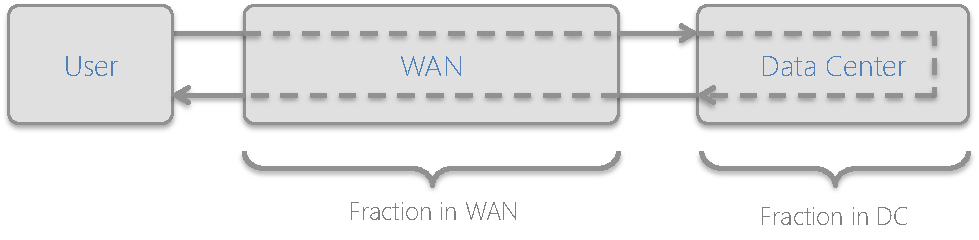
\includegraphics[width=\linewidth]{../figs/DC_model.pdf}
  \caption{Typical User-DC communication pattern}
  \label{fig:DC_model}
\end{figure}

We have chosen Google Search as a representative user-facing service for our case study. One reason for choosing Google Search is that the service provides a metric of estimated time spent within the DC (Fig.\,\ref{fig:google_time}). From our analysis in Sec.\,\ref{sec:analysis}, we believe this data to be fairly accurate in reflecting the fraction of round-trip time spent inside the DC.

\begin{figure}[t]
  \centering
  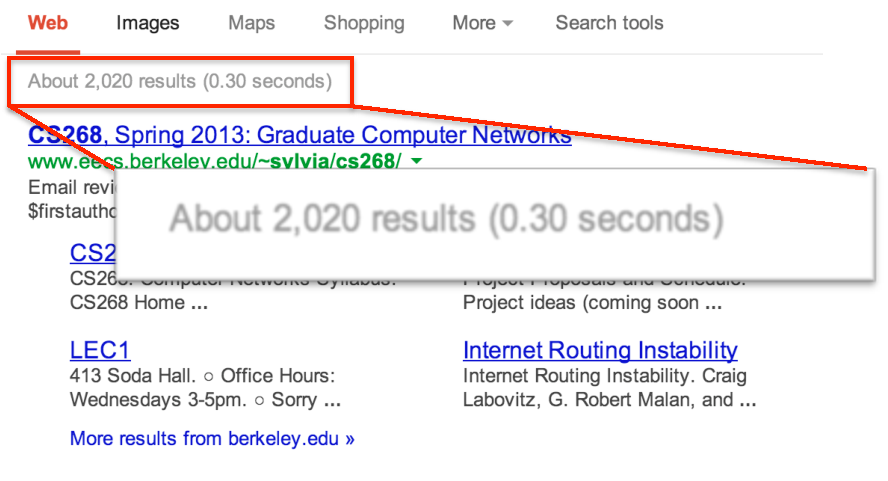
\includegraphics[width=0.85\linewidth]{../figs/GoogleTime.pdf}
  \caption{Google Search estimated time spent within DC as presented in the search results page}
  \label{fig:google_time}
\end{figure}

We perform a query at the end-host and time-stamp the start and end times. In this way we can measure the complete round-trip time for a single query as experienced by the end-host. The largest hurdle is selecting a search term to query. Initially, we suspected that caching within the DC would impact our results. Thus, we believed that "hot trends" (Google's own reported highest searched terms) were likely to be cached. As such, they would provide a baseline measurement for understanding the WAN latency as minimal time spent would be spent within the DC. On the other hand, we use a random string in our  queries minimize the probability of caching and force the query to be processed. We extracted "hot trends" from Google Trends\footnote{http://www.google.com/trends/hottrends}, and we generate random strings of length 32, comprised of numbers and letters (both lower and uppercase). Our analysis in Sec.\,\ref{sec:analysis} shows that the results of our measurements produced differed greatly from our original assumptions. Nonetheless, we believe this methodology is useful in understanding the fraction of round-trip time spent inside the DC.

To provide context for our measurements, we perform \texttt{ICMP ping} queries to measure the network latency from the end-user to Google. Because we conduct this experiment in a geographically distributed fashion and because Google has many user-facing servers/IPs, we must take additional steps to ensure the server being pinged is in fact responsible for handing our search queries. We process the application layer HTTP conversation at the using \texttt{tcpdump} to capture all the packets and extract the IP of the Google server.
 
In Table \ref{tab:DC_method} we provide an overview of the four different ``time'' measurements derived from our experiment. One thing to notice is that Google time is present only when the query makes sense to Google. For the random 32-character long string, there is no Google time. 

\begin{table}
  \begin{tabular}{p{2.8cm} | p{5cm}}
    \hline
    type & description \\
    \hline
    Hot-trend-query time & the time spent to query a hot trend word to Google. \\
    Random-query time & the time spent to query a 32-character random string.  \\
    Ping time & the networking layer round-trip time to the responded Google IP address. \\
    Google time & Google's own estimated time spent within their DC. \\
    \hline
  \end{tabular}
  \vspace{1em}
  \caption{Four different ``times'' measured}
  \label{tab:DC_method}
\end{table}


% \begin{itemize}
% \setlength{\leftmargin}{-1pt}
% \setlength{\itemsep}{1pt}
% \setlength{\parskip}{0pt}
% \setlength{\parsep}{0pt}
% \item Hot-trend-query time \\
%   the time spent to query a hot trend word to Google. 
% \item Random-query time -- the time spent to query a 32-character random string. 
% \item Ping time -- the networking layer round-trip time to the responded Google IP address.
% \item Google time -- Google's estimated time spent within their DC.
% \end{itemize}


\subsection{Implementation and Experiment}
\label{sec:impl-exper}

We implemented our measurement script in Python, and use \texttt{cron} to schedule the execution every two hours. In each pass, the script will first visit Google Trends webpage and obtain the hot-trend words for that hour. Along with randomly generated strings, we create a list of 20 strings to query. The entire list is queried repeatedly 10 times, and the four ``times'' are recorded. Each query is conducted using Python urllib2 library over HTTP, using the query address \url{http://www.google.com/search?hl=en\&output=search\&q=query}.\footnote{One thing to note about our implementation is that it violates Google's terms of service, as sending automated queries is disallowed. In the event automated queries are detected, Google responds with a page containing the following message: ``Our systems have detected unusual traffic from your computer network.'', and the users will be required to enter a CAPTCHA. The workaround we utilize is to limit the query speed. So after each query, we delay the script for 5 seconds. We should point out that there are at most $12\times10\times20$ queries per node per day, which limits our sample size.}

While performing a query, we utilize \texttt{tcpdump} to monitor the incoming and outgoing traffic on port 80. By inspecting the TCP traces, we can find the specific Google IP that responds our query. We then \texttt{ping} this IP 10 times and record the results. \texttt{tcpdump} and \texttt{ping} are invoked using Python subprocess module.

We deployed the code on 19 PlanetLab nodes, however only 13 of them are running correctly during the measurement period (Apr.\,18 - Apr.\,25).

\subsection{Analysis}
\label{sec:analysis}

In Fig.\,\ref{fig:data_center}, we put all the obtained results in single plot. On the left, we show the median value of random query time, hot-trend query time, google time and ping time. On the right, we divide the Google time by hot-trend query time to calculate the Google portion. The average value for each node is plotted on the right.

First, we noticed that random query is usually taking less time than hot-trend query. This contradicts with our initial thinking about caching. It seems that all these queries are not cached by Google's user-facing servers. Any single query goes into their Data Center. And it's easier to return search value when the query is random string, while regular words would take longer time to process. Since Google guarantees the search results to be fresh, for hot-trend words, though there are so many people searching, there is also a high chance some new pages about these words appear. So having the search processed by their DC can provide better search experience to the public.

Another thing to notice is that though the ping time, and query time varies a lot across these test points, the Google time is relatively stable (around 0.2 seconds). So the Google portion's variation is primarily determined by the WAN performance. For ``6test.edu.cn'' machine in China, each single query takes about 1 second to finish, making the Google portion around 22\%. But generally the time within WAN and DC are fairly close for an end-user, which means that optimization on either side would benefit the user.

\begin{figure*}[!htb]
  \centering
  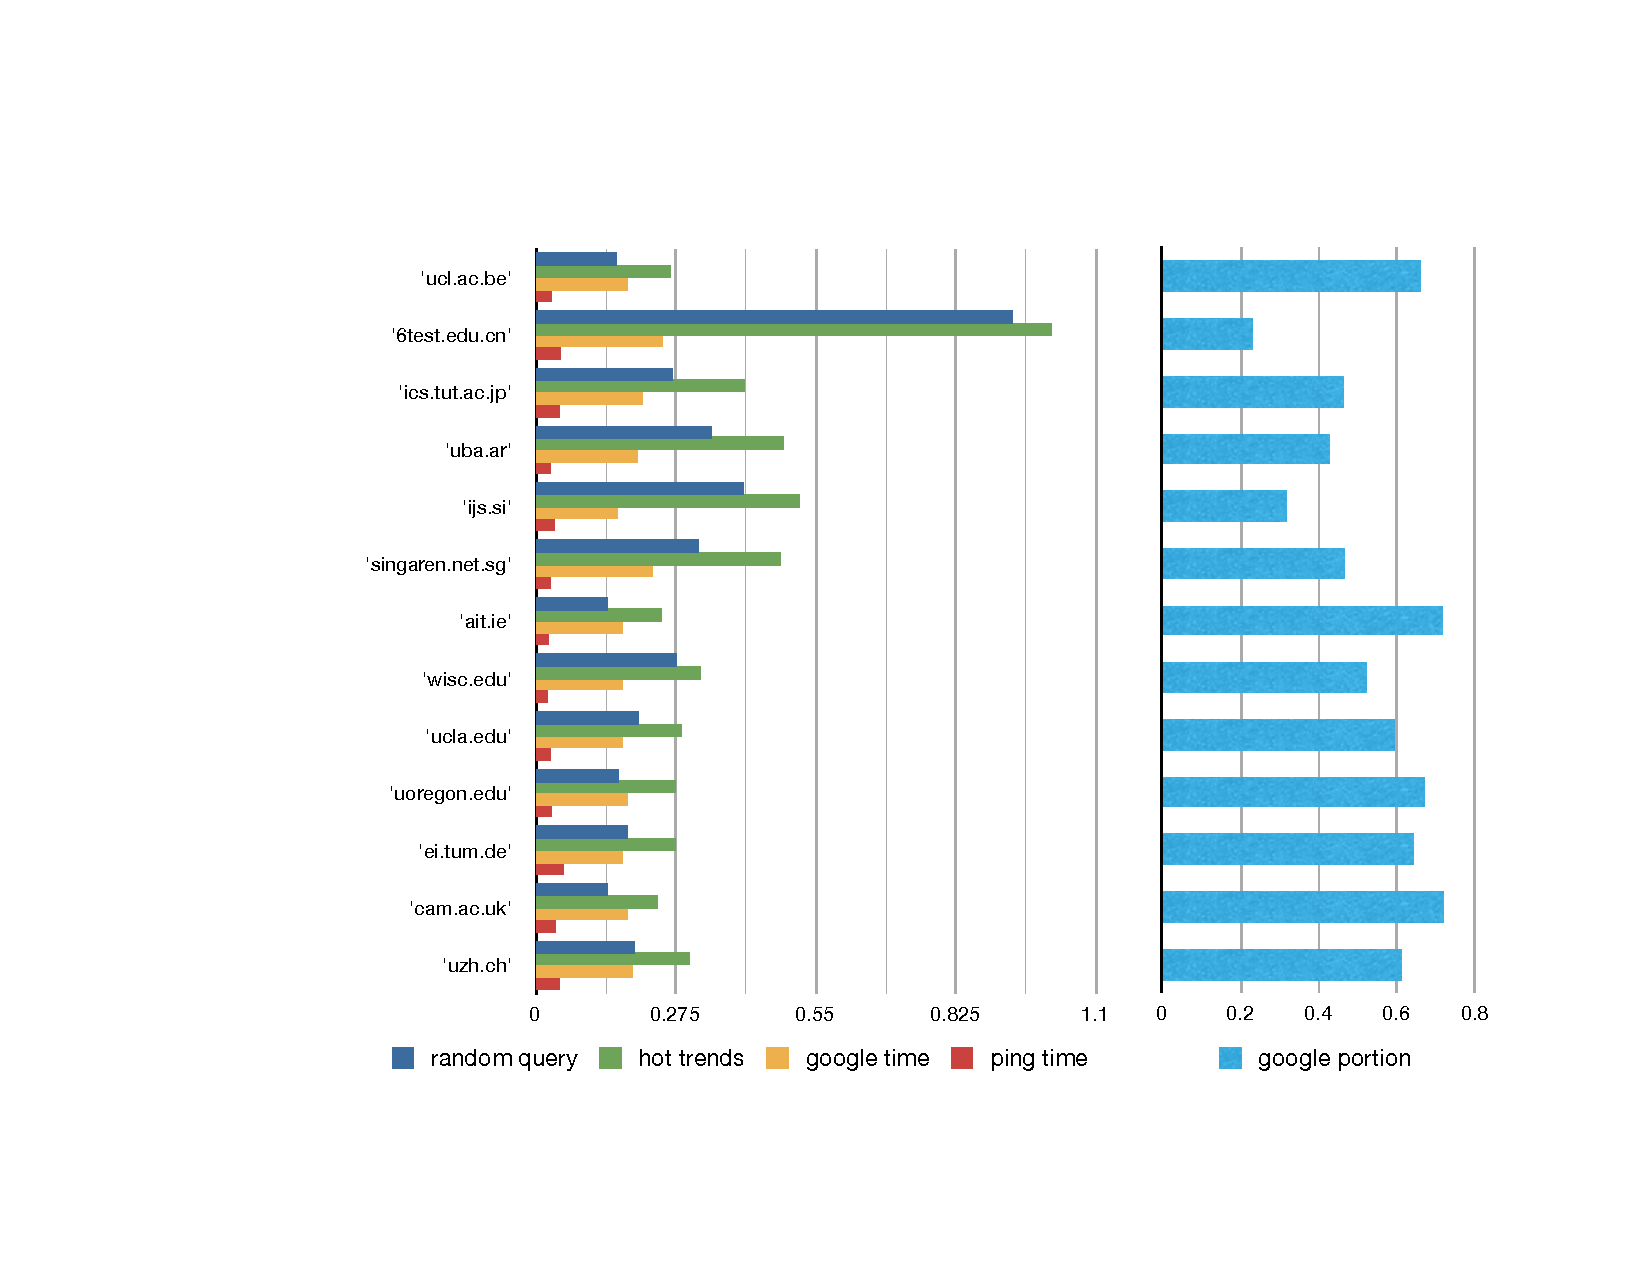
\includegraphics[width=\linewidth]{../figs/data_center.pdf}
  \caption{(Left) Four different ``times'' in our DC vs. WAN experiement. (Right) The average of Google time portion within a query conversation for each PlanetLab node test point.}
  \label{fig:data_center}
\end{figure*}

We further asked ourself questions like ``what if the networking latency is so small, how large the benefit might be?''. For this, we haven't really done too much analysis, but we will present some preliminary results using one of the \texttt{tcpdump} example (Fig.\,\ref{fig:tcpdump}. 

\begin{figure}[!htb]
  \centering
  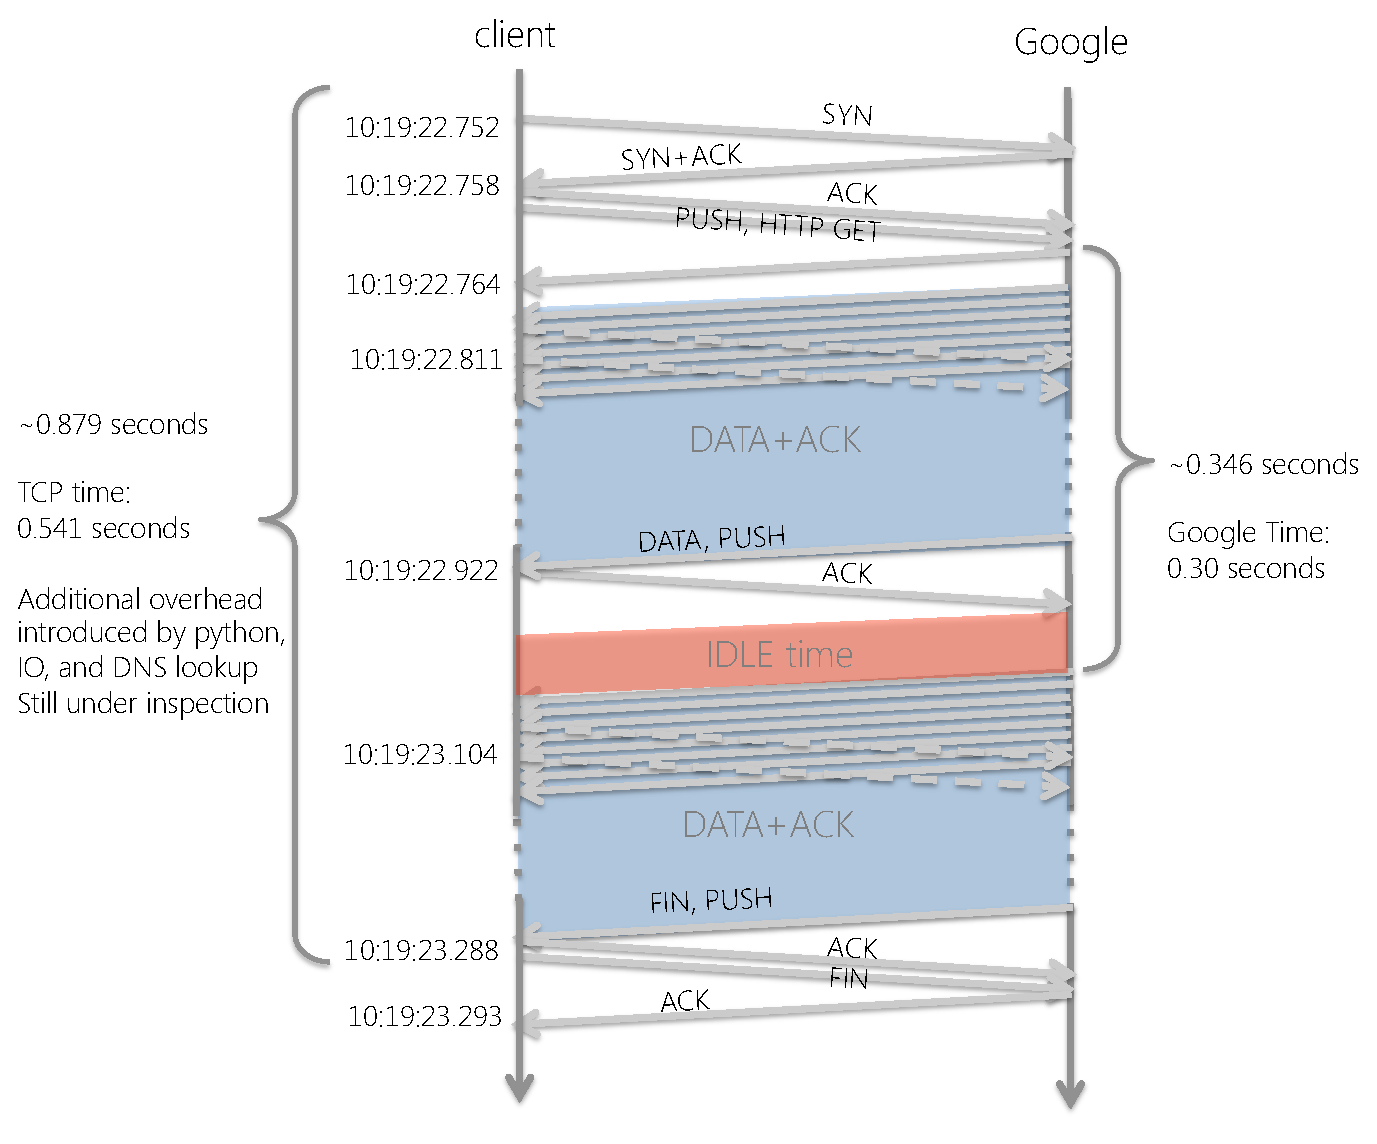
\includegraphics[width=\linewidth]{../figs/tcpdump.pdf}
  \caption{One example \texttt{tcpdump} analysis in Google query}
  \label{fig:tcpdump}
\end{figure}

This trace is collected in Berkeley EECS-secure wireless network when we search ``CS268''. The \texttt{ping} time to Google is around 5 ms. For the trace, we annotated with the time like ``10:19:22.752'' for illustration. As a typical HTTP (TCP) conversation, after the three-way handshake, the client sends out the query -- HTTP GET, the server then responds with the data. For DC-involved services, this might delay for some time since the query has be to processed. However, the server might take another strategy, like what Google is doing -- it can send out part of the final results first (either javascript or CSS part). Then when the task is finished inside DC, the rest of the results are sent back. Each return page from Google Search is around 200KB, and separating them can largely reduce the amount of overall latency experienced by end-user. 

From this graph, one possible argument is that if we optimize the DC performance hard, reducing the Google Time, what we end up with is reducing the idle time shown in the figure. It's actually not a huge portion of the whole HTTP conversation, especially this is when the average network latency to Google is around 5 ms. For those end hosts who have a worse network connection, the IDLE time portion will be even larger. Additional experiements are needed to validate such argument, and we put that into our future work.

%%% Local Variables: 
%%% mode: latex
%%% TeX-master: "main"
%%% End: 

